\chapter{Introduction}

Here, we'll dive into the basics of the Shape Diameter Function (SDF), which is a really fancy way of figuring out how thick or thin a 3D object is. We'll explore what the SDF is, why we care about it, how others have tried to compute it using GPUs, and what we're going to achieve in this thesis.

\section{Context}

But what exactly is the Shape Diameter Function? Introduced by Shapira et al.\ \cite{shapira2008}, you can think of the SDF as a tool that measures the "thickness" of a 3D model at any given point on its surface. Imagine you are standing on the surface of a 3D model at a specific point $p$. If you look straight down into the object (along the negative normal $-\vec{\mathbf{n}}$), how deep is it before you pop out the other side? That depth is essentially what the SDF measures!

However, just measuring a single straight line can give us wonky results if the object is bumpy inside. To solve this, we don't just shoot one straight line. Instead, we shoot a whole "cone" of rays inward from point $p$. We measure how far each ray travels before hitting the opposite wall, and then we calculate the average of all those distances:

\begin{equation}
    \text{SDF}(p) = \frac{\sum_{i=1}^{R} d_i \cdot w_i}{\sum_{i=1}^{R} w_i}
\end{equation}

\begin{figure}[H]
\centering
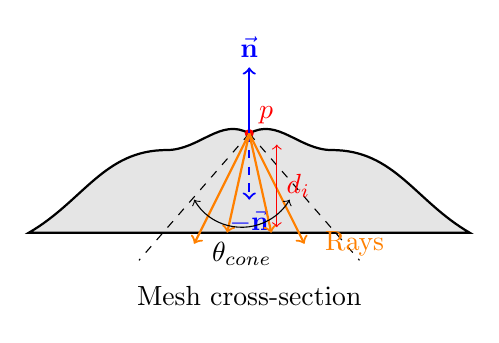
\begin{tikzpicture}[scale=0.7]
    % Draw mesh surface (cross-section)
    \draw[thick, fill=gray!20] (-4,0) to[out=30,in=180] (-1.5,1.5) to[out=0,in=150] (0,1.8) to[out=30,in=180] (1.5,1.5) to[out=0,in=150] (4,0) -- cycle;
    
    % Point p on surface
    \filldraw[red] (0,1.8) circle (2pt) node[above right] {$p$};
    
    % Normal vector (outward)
    \draw[blue, thick, ->] (0,1.8) -- (0,3.0) node[above] {$\vec{\mathbf{n}}$};
    
    % Inverted normal (inward)
    \draw[blue, thick, ->, dashed] (0,1.8) -- (0,0.6) node[below] {$-\vec{\mathbf{n}}$};
    
    % Cone boundary lines (dashed)
    \draw[dashed] (0,1.8) -- (-2.0,-0.5);
    \draw[dashed] (0,1.8) -- (2.0,-0.5);
    
    % Cone of rays (solid orange)
    \draw[orange, thick, ->] (0,1.8) -- (-1.0,-0.2);
    \draw[orange, thick, ->] (0,1.8) -- (-0.4,0.0);
    \draw[orange, thick, ->] (0,1.8) -- (0.4,0.0);
    \draw[orange, thick, ->] (0,1.8) -- (1.0,-0.2);
    
    % Distance annotation (along one ray)
    \draw[red, <->] (0.5,1.6) -- (0.5,0.1) node[midway, right] {$d_i$};
    
    % Cone angle arc
    \draw[<->] (-1.0,0.6) arc[start angle=210,end angle=330,radius=1.0] node[midway, below=2pt] {$\theta_{cone}$};
    
    % Labels
    \node[below] at (0,-0.8) {Mesh cross-section};
    \node[orange, right] at (1.2,-0.2) {Rays};
\end{tikzpicture}
\caption{Illustration of the SDF computation.}
\label{fig:sdf_concept}
\end{figure}

Figure~\ref{fig:sdf_concept} shows a visual breakdown of this process. A cone of rays is shot inward from point $p$. Each ray travels until it hits the opposite wall, recording its travel distance $d_i$. But are all rays treated equally? Nope! Rays shooting straight down the middle are usually more accurate than rays shooting out at wide angles ($\theta_i$). Because of this, we give the straighter rays a higher "weight" ($w_i$). The final SDF value is just the average of these weighted distances (typically using $R = 64$ rays).

As you might guess, a thick area (like a person's torso) will have very long ray distances, resulting in a large SDF value. However, a thin area (like a finger or an ear) will have very short ray distances, resulting in a small SDF value. Because this measurement relies purely on the object's volume, you can spin the object around or bend its arms and legs, and the thickness values won't change!

\begin{figure}[ht]
\centering
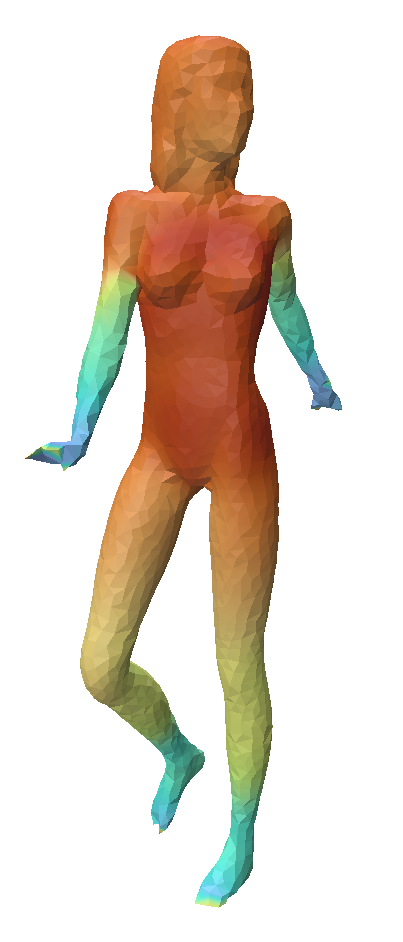
\includegraphics[width=0.45\textwidth]{images/Chapter3/Introduction/Torso.PNG}
\caption{A 3D model of a human torso SDF value heatmap.}
\label{fig:torso}
\end{figure}

Figure~\ref{fig:torso} shows a 3D model of a human torso. The SDF values are highest in the chest and abdomen regions, where the volume is thickest, and decrease toward the neck and shoulders.

\section{Why SDF: Role in 3D Object Analysis}

But why do we care about how thick a 3D model is? It turns out that knowing an object's thickness is incredibly useful for computers! For example, it helps with mesh segmentation (cutting a 3D model into logical pieces, like separating an arm from a body because the wrist is thinner), skeletonization (finding the "bones" inside a 3D character by tracing the thickest parts), and even character animation (figuring out how a 3D character should bend and move naturally).

However, there is a catch. Figuring out the thickness for millions of points on a highly detailed 3D model takes a massive amount of math. Doing this on a standard computer processor (CPU) is agonizingly slow. This bottleneck led researchers to start moving the math over to graphics cards (GPUs), which are amazing at doing thousands of tiny math problems at the exact same time.

\section{Survey of Existing Work}

Several approaches have been developed for computing the SDF on the GPU.

\subsection{PyMeshLab GPU (VCGlib)}

PyMeshLab uses a trick with computer graphics (OpenGL) called the ``spawning camera'' technique \cite{vcglib}. Think of it like placing virtual security cameras all around the 3D object. Each camera takes a picture of how deep the object looks from its specific angle. By blending all these pictures together, it figures out the overall thickness!

But there's a problem with this. Setting up all these virtual cameras and combining their pictures requires a lot of setup time. Because of this heavy setup, even tiny, simple 3D models still take at least 0.3 seconds to process.

\subsection{Kamenick\'{y} -- OpenCL Parallelization}

Kamenick\'{y} \cite{kamenicky2014} tried a different approach using OpenCL (a tool that lets programs run on different types of graphics cards). They proved that if you shoot the rays in parallel using the GPU, you get a massive speed boost over traditional CPU methods.

However, OpenCL is a bit of a ``jack of all trades.'' It works on many devices, but it misses out on the specialized, ultra-fast ray tracing hardware (like RT Cores) built into modern NVIDIA cards.

\subsection{Fast and Robust Shape Diameter Function}

Chen et al.\ \cite{chen2018} realized that shooting dozens of rays from every single point was slow and sensitive to bumpy, noisy surfaces. So, they wrapped the whole 3D model in a smooth virtual bubble (an ``offset surface''). By measuring from this smooth bubble instead of the bumpy surface itself, they only needed to shoot a single ray per point! This clever trick made the process about 10 times faster and handled broken or noisy 3D models perfectly.

\section{Objective}

So, where do we fit into all of this? The main goal of this thesis is to build the ultimate, high-speed SDF calculator using modern High Performance Computing. Specifically, we aim to build a super-fast pipeline using NVIDIA OptiX to take full advantage of specialized ray tracing hardware (RT Cores), pit our new OptiX approach against the existing PyMeshLab camera-trick method to see who wins in speed and accuracy, and prove that using dedicated ray tracing hardware is the best way to compute 3D thickness.

Now that we know what we're building and why, the next chapter will introduce the awesome tools we'll be using to make it happen (like NVIDIA OptiX and CUDA).
